\documentclass[12pt,british,VeneziaPhdThesis]{PhdThesis}[2004/02/17]%,draft

\newcommand\hmmax{0}
\newcommand\bmmax{0}

\usepackage{babel}

\usepackage[ruled]{algorithm2e}
\usepackage{algpseudocode}
\usepackage{amsmath,amsthm,amssymb}
\usepackage{amsmath}
\usepackage{amsfonts}
\usepackage{amssymb}
 
\usepackage{amsthm}
\usepackage{amsxtra}
 
\usepackage{babel}
\usepackage{bm,overpic}
\usepackage{booktabs}
 
\usepackage{braket}
 
\usepackage{cite}
\usepackage{color}
 
\usepackage{comment}
\usepackage{epigraph}
\usepackage{epstopdf}
\usepackage{enumitem}
\usepackage[mathscr]{eucal}

\usepackage{float}
 
\usepackage{fourier}
\usepackage{graphicx} 
\usepackage{subcaption}
 
\graphicspath{{Pictures/}} % Specifies the directory where pictures are stor

\usepackage{epsfig}

\usepackage{longtable}
\usepackage{lscape}
\usepackage{mathrsfs}

\usepackage{mathtools}
\usepackage{multirow}
\usepackage{multicol}
\usepackage{makecell}
\renewcommand\cellset{\renewcommand\arraystretch{0}%
\setlength\extrarowheight{0pt}}
\usepackage{physics}

%\usepackage{pdfpages}
\usepackage{multibib}
%\newcites{pri}{Bibliography}
\newcites{sec}{Published Papers}
 

\usepackage{pdfpages}

\usepackage{placeins}
\usepackage{pseudocode}

\usepackage{textcomp}
\usepackage{tikz}
\usepackage{times}
%\usepackage{todo}
\usepackage{url}

% for frontespizio
\usepackage{eso-pic}
 



%\usepackage[cal=lucida]{mathalfa}
%\usepackage{CJKutf8}
%\usepackage{algorithmic}
%\usepackage{algorithm}

%\setcounter{tocdepth}{3}
\setcounter{secnumdepth}{4}

\usetikzlibrary{arrows,shadows}


% here more packages

%this only if you like to use some of its features (like smartrefs)
% \usepackage{theorems}[2003/12/05]

% consider to use hyperref
\usepackage[bookmarks=true,bookmarksopen=true,pdfhighlight=/I,pdfpagemode=UseOutlines,linktocpage,hidelinks]{hyperref}%if you use pdflatex
% \usepackage[hypertex, colorlinks=true, backref]{hyperref}%if you use latex
\usepackage{url}
\usepackage{caption}

% learn to use includes! 
% \includeonly{introduction,preliminaries}


%\usepackage[refpages]{gloss} %per compilare bibtex phdthesis.gls.aux
 
\def\R{ \hbox{I\kern-.1667em R}}
\def\Tr{\mathrm{Tr}}
\def\tr{\mathrm{Tr}}
%\newcommand{\R}{\mathbb{R}}
\newcommand{\T}{^T}
\newcommand{\argmax}{\operatornamewithlimits{\arg\,\max}}
%\newcommand{\bm}[1]{\boldsymbol{\mathrm{#1}}}
\newcommand{\dom}{\mathrm{dom}}
%\newcommand{\dquote}[1]{``#1''}
%\newcommand{\e}{\vct{1}}
%\newcommand{\gvct}[1]{\boldsymbol #1}
\newcommand{\half}{{\textstyle \frac{1}{2}}}
\newcommand{\hide}[1]{}
\newcommand{\mat}[1]{\begin{pmatrix}#1\end{pmatrix}}
\newcommand{\todo}[1]{\textbf{#1}}
\newcommand{\vct}[1]{\mathbf #1}
%\newcommand{\vct}[1]{\mbox{\boldmath$#1$}}
\newcommand{\x}{\vct{x}}
\newcommand{\y}{\vct{y}}
\newcommand{\fracpartial}[2]{\frac{\partial #1}{\partial  #2}}
\newcommand{\inlineeqnum}{\refstepcounter{equation}~~\mbox{(\theequation)}}
\newcommand{\ith}[1]{$#1$-th}
 


\newtheorem{conjecture}{Conjecture}
\newtheorem{corollary}{Corollary}
\newtheorem{definition}{Definition}
\newtheorem{lemma}{Lemma}
\newtheorem{proposition}{Proposition}
\newtheorem{theorem}{Theorem}

\renewcommand{\vec}[1]{\mathbf{#1}}


%%\newtheoremstyle{example}{.6cm}{.6cm}%
%%     {}%         Body font
%%     {}%         Indent amount (empty = no indent, \parindent = para indent)
%%     {\bfseries}% Thm head font
%%     {}%        Punctuation after thm head
%%     {\newline}%     Space after thm head (\newline = linebreak)
%%     %{\thmname{#1}\thmnumber{ #2}\thmnote{ #3}}%         Thm head spec
%%     {\thmname{#1}\thmnumber{ #2}\thmnote{ #3}}%         Thm head spec
%%
%%\theoremstyle{example}
%%\newtheorem{example}{Example}[section]

% Alter some LaTeX defaults for better treatment of figures:
% See p.105 of "TeX Unbound" for suggested values.
% See pp. 199-200 of Lamport's "LaTeX" book for details.
%   General parameters, for ALL pages:
\renewcommand{\topfraction}{0.9}	% max fraction of floats at top
\renewcommand{\bottomfraction}{0.8}	% max fraction of floats at bottom
%   Parameters for TEXT pages (not float pages):
\setcounter{topnumber}{2}
\setcounter{bottomnumber}{2}
\setcounter{totalnumber}{4}     % 2 may work better
\setcounter{dbltopnumber}{2}    % for 2-column pages
\renewcommand{\dbltopfraction}{0.9}	% fit big float above 2-col. text
\renewcommand{\textfraction}{0.07}	% allow minimal text w. figs
%   Parameters for FLOAT pages (not text pages):
\renewcommand{\floatpagefraction}{0.7}	% require fuller float pages
% N.B.: floatpagefraction MUST be less than topfraction !!
\renewcommand{\dblfloatpagefraction}{0.7}	% require fuller float pages
\renewcommand{\textfraction}{0.05}
\renewcommand{\topfraction}{0.95}
\renewcommand{\bottomfraction}{0.95}
\renewcommand{\floatpagefraction}{0.9}

\newcommand{\etal}{\textit{et al}. }
\newcommand{\ie}{\textit{i}.\textit{e}., }
\newcommand{\eg}{\textit{e}.\textit{g}., }
\newcommand{\etc}{\textit{etc}. }
\newcommand{\wrt}{with respect to }
\newcommand*\cleartoleftpage{%
  \clearpage
  \ifodd\value{page}\hbox{}\newpage\fi
}


% Import pxtx package calling with \mtxcal
% https://tex.stackexchange.com/a/500774/216100
\DeclareFontFamily{U}{txcal}{\skewchar \font =45}
\DeclareFontShape{U}{txcal}{m}{n}{
<-> txr-cal}{}
\DeclareFontShape{U}{txcal}{b}{n}{
<-> txb-cal}{}
\DeclareMathAlphabet{\mtxcal}{U}{txcal}{m}{n}
\SetMathAlphabet{\mtxcal}{bold}{U}{txcal}{b}{n}
\DeclareMathAlphabet{\mtxbcal} {U}{txcal}{b}{n}

\newcommand{\Graph}{\mtxcal{G}}
\usepackage{chapters/utility/results/lvae}
 

%\makegloss  

\author{Mark Lion}
\cycle{3X}
\accyearstart{2020/2021}
\accyearend{2022/2023}
\matriculation{8XXXXX}
\sector{INF/01}
\email{mark.lion@unive.it}
% \homepage{\url{http://www.dais.unive.it/~minello}}

\supervisor{Prof. God}
\phdcoord{Prof. God supreme}
\title{Awesome research}
\date{September, 202X}
\phdnumber{}

\makeindex

\begin{document}
\renewcommand{\chapterautorefname}{Chapter}
\renewcommand{\sectionautorefname}{Section}
\renewcommand{\subsectionautorefname}{Section}

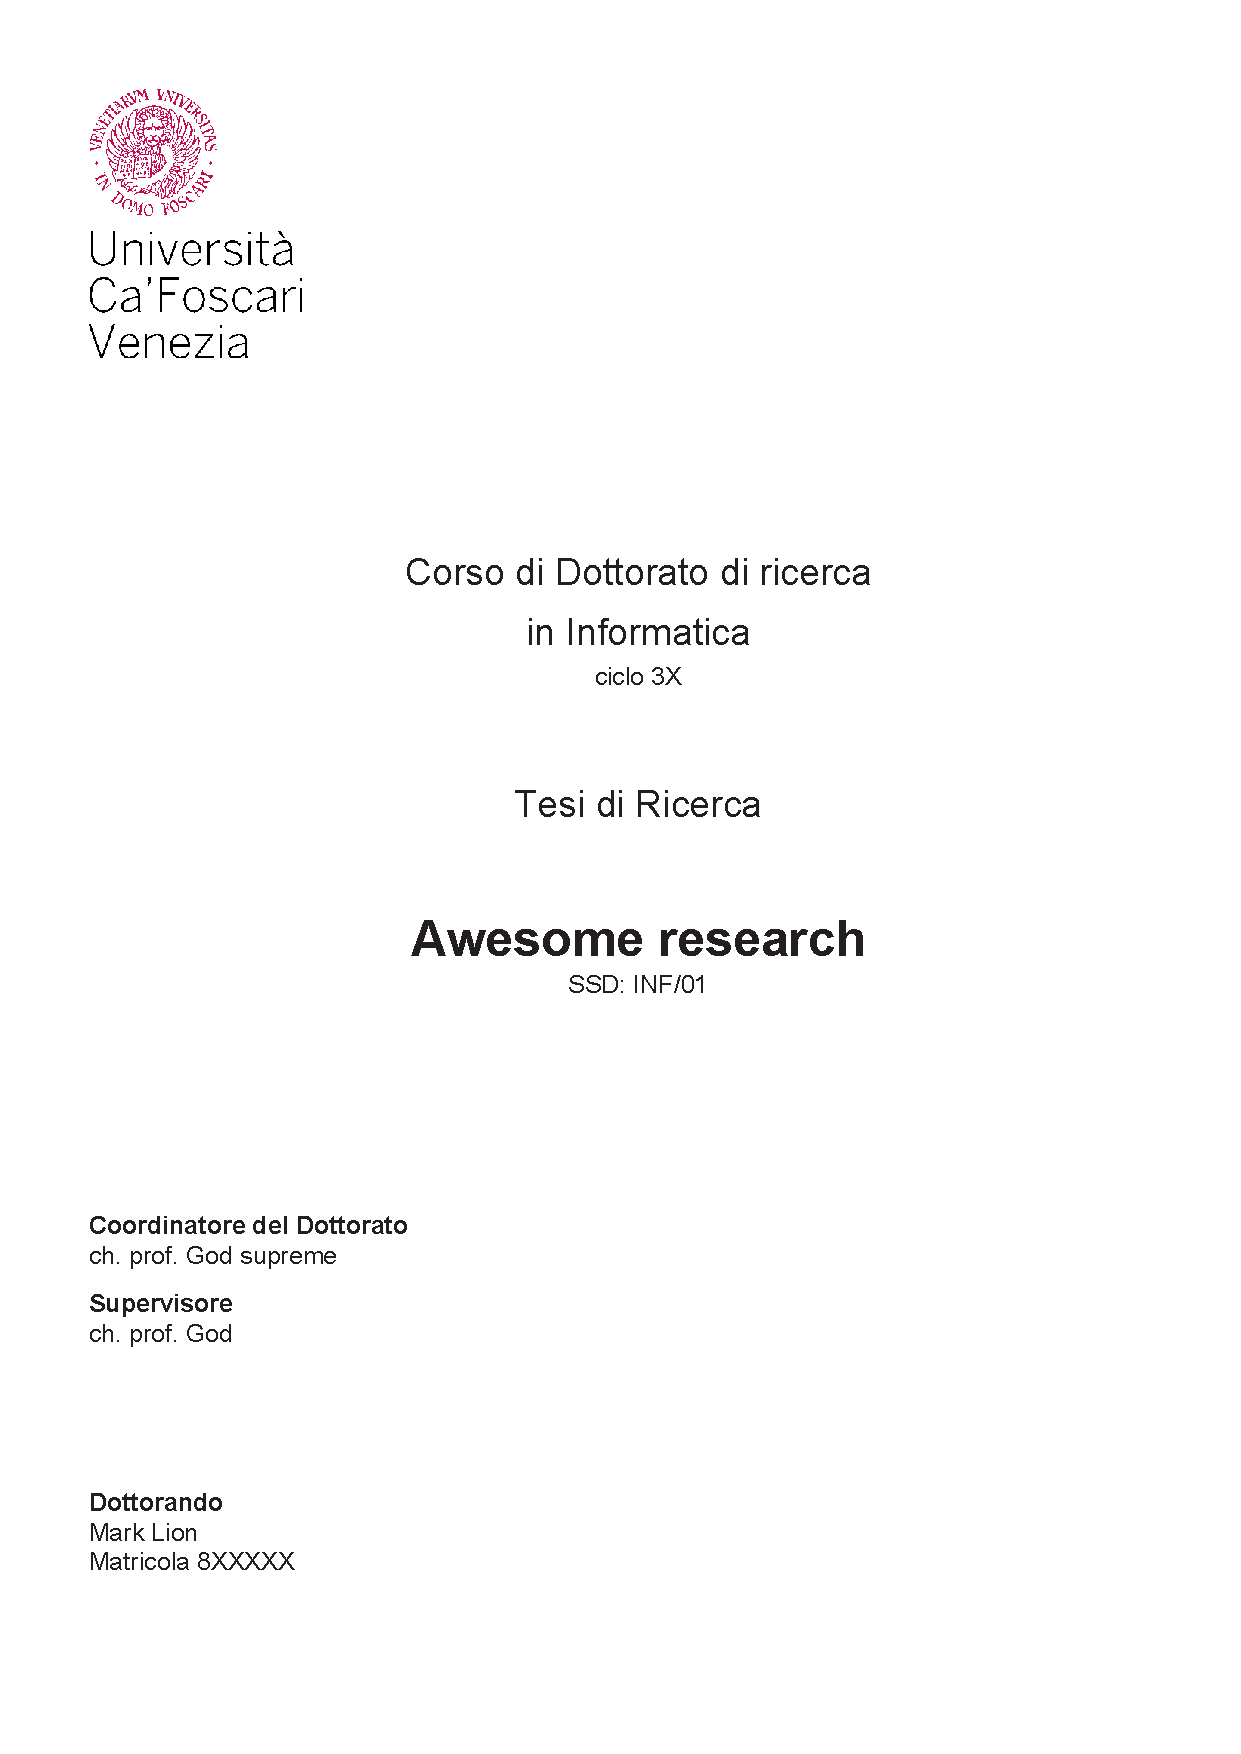
\includepdf{frontespizio_tesi_dottorati.pdf}

 

\pagestyle{empty}
\maketitle
\begin{abstract}

ABSTRACT 

Lorem ipsum dolor sit amet, consectetur adipiscing elit. Nam et rhoncus arcu, at finibus augue. Curabitur sollicitudin metus ut enim eleifend dictum. Nunc ultricies varius eros nec bibendum. Duis et aliquam nulla. Vivamus consequat ligula et augue vehicula, ut ultrices ex porttitor. Donec diam justo, vehicula faucibus erat et, sodales vehicula dolor. Curabitur at aliquet lectus. Fusce facilisis sollicitudin nisi vel fermentum.

Curabitur nec vestibulum lorem. Sed vehicula sapien fermentum, interdum ante nec, facilisis est. Morbi aliquam tempus lectus. Curabitur ac rhoncus augue, eget scelerisque nisl. Quisque pulvinar gravida suscipit. Sed enim quam, lacinia eget nisl et, iaculis feugiat ex. Donec mi nulla, condimentum nec turpis sed, mattis pharetra nibh. Maecenas mattis, erat a volutpat blandit, ante elit vulputate lectus, eu cursus dui quam in turpis. Aliquam lacinia, quam id cursus condimentum, nisl lorem porttitor urna, non dapibus magna quam eget felis.
 
\end{abstract}
\label{abstract}

%\chapter*{Sommario}
%
%Lorem ipsum dolor sit amet, consectetur adipisci elit, sed eiusmod tempor incidunt ut labore et dolore magna aliqua. Ut enim ad minim veniam, quis nostrum exercitationem ullam corporis suscipit laboriosam, nisi ut aliquid ex ea commodi consequatur. Quis aute iure reprehenderit in voluptate velit esse cillum dolore eu fugiat nulla pariatur. Excepteur sint obcaecat cupiditat non proident, sunt in culpa qui officia deserunt mollit anim id est laborum.

\frontmatter
\partstyle{serifbig}
\chaptertitlestyle{serifbig}
\pagestyle{serif}
\tableofcontents
\listoffigures

 


%
%\nocitesec{*}
%\bibliographystylesec{acm}
%\bibliographysec{sec_bib}

%\printgloss{notation}  %RIMUOVERE PER GLOSSARIO
%\nocitemypub{*}
%\bibliographystylemypub{acm} %
%\bibliographymypub{sec_bib.bib}



\newenvironment{myindentpar}[1]%
 {\begin{list}{}%
     {\setlength{\leftmargin}{#1}}%
     \item[]%
 }
 {\end{list}}


\begin{preface}

Lorem ipsum dolor sit amet, consectetur adipiscing elit. Nam et rhoncus arcu, at finibus augue. Curabitur sollicitudin metus ut enim eleifend dictum. Nunc ultricies varius eros nec bibendum. Duis et aliquam nulla. Vivamus consequat ligula et augue vehicula, ut ultrices ex porttitor. Donec diam justo, vehicula faucibus erat et, sodales vehicula dolor. Curabitur at aliquet lectus. Fusce facilisis sollicitudin nisi vel fermentum.

Curabitur nec vestibulum lorem. Sed vehicula sapien fermentum, interdum ante nec, facilisis est. Morbi aliquam tempus lectus. Curabitur ac rhoncus augue, eget scelerisque nisl. Quisque pulvinar gravida suscipit. Sed enim quam, lacinia eget nisl et, iaculis feugiat ex. Donec mi nulla, condimentum nec turpis sed, mattis pharetra nibh. Maecenas mattis, erat a volutpat blandit, ante elit vulputate lectus, eu cursus dui quam in turpis. Aliquam lacinia, quam id cursus condimentum, nisl lorem porttitor urna, non dapibus magna quam eget felis.

Aliquam elementum erat non rhoncus porttitor. Sed dictum placerat mi, ac aliquam libero. Aliquam enim ante, egestas quis dui quis, pretium blandit urna. Nam eu sem tortor. Maecenas facilisis, lectus vel aliquet dignissim, quam enim pulvinar lacus, suscipit euismod ligula augue blandit magna. Vivamus pellentesque, mauris at convallis commodo, lacus nisi sollicitudin libero, sit amet dictum dui tortor quis quam. Interdum et malesuada fames ac ante ipsum primis in faucibus. Maecenas id nulla efficitur, pellentesque augue in, maximus lacus. Etiam posuere pellentesque convallis. Curabitur malesuada laoreet pharetra. Fusce quis eros accumsan, tincidunt quam nec, tempus nibh. Vestibulum non neque elementum, blandit erat nec, fermentum nulla.

Duis egestas nunc vitae scelerisque vestibulum. Quisque luctus lectus non porttitor sodales. Praesent nec mauris non magna porta venenatis vitae et eros. Maecenas non nunc sed leo hendrerit lobortis nec eget tortor. Etiam finibus dignissim justo id ultrices. Pellentesque habitant morbi tristique senectus et netus et malesuada fames ac turpis egestas. In feugiat consectetur tincidunt.

Praesent at est pellentesque, accumsan nulla eu, condimentum odio. Vestibulum in ex tincidunt, tincidunt neque eu, elementum arcu. Vivamus mauris augue, rhoncus eu consequat ut, vulputate non dolor. Mauris accumsan sagittis felis, vel porta quam aliquet quis. Donec porttitor sed ipsum in faucibus. Proin quis porttitor nibh, sit amet imperdiet orci. Cras blandit, arcu a hendrerit convallis, est sapien vestibulum enim, sed interdum orci odio at ligula. In pretium euismod lectus eget lacinia. Etiam feugiat hendrerit neque ac tempor. In nunc erat, ornare vitae tortor facilisis, sollicitudin ullamcorper metus. Integer eu rutrum lectus. Donec et commodo tellus. Donec pulvinar risus ex. Vestibulum vel odio metus. Curabitur finibus nibh mattis diam lobortis, sed pulvinar nulla eleifend.

\end{preface}



\nocitesec{*}
\bibliographystylesec{acm}
\bibliographysec{sec_bib}
%%\addcontentsline{toc}{chapter}{Bibliografia}

\hide{
\chapter*{Notations
\chaptermark{Notations}\sectionmark{Notations}}
\setcounter{section}{0}%
\setcounter{subsection}{0}%
\addcontentsline{toc}{chapter}
{\protect\numberline{}Notations}%
\thispagestyle{empty}

%\begin{tabular*}{\textwidth}{ll@{\extracolsep{\fill}}r}
%\setlength\LTleft{0pt}
%\setlength\LTright{0pt}
\begin{longtable}{ll@{\extracolsep{\fill}}r}
\multicolumn{3}{l}{\bf General}\\
\hline
$\mathbb R$& set of reals&\\
$\mathbb R_+$& set of nonnegative reals&\\
$|S|$&cardinality of the set $S$&\\
$\vct x$, $\vct y$, $\vct z$,\dots&column vectors in $\mathbb R^n$&\\
$x_i$&$i$th element of vector $\vct x$&\\
$\vct 0$&column vector of all 0s&\\
$\vct e$&column vector of all 1s&\\
$\vct e^i$&$i$th column of the identity matrix&\\
$A=(a_{ij})$&matrix in $\mathbb R^{n\times n}$ with $(i,j)$th element $a_{ij}$&\\
$I$&identity matrix&\\
$det(A)$&determinant of matrix $A$&\\
$\binom{V}{k}$&set of $k$-subsets of $V$&\\
&&\\
\multicolumn{3}{l}{\bf Game-theory}\\\hline
$S=\{1,\dots,n\}$&set of $n$ strategies usually denoted with $S$\\
$\Delta^n$&standard simplex in $n$ dimensions&\\
$\pi(\vct y|\vct x)$&$\vct y^TA\vct x$, average payoff of $\vct y$ against $\vct x$\\
$\pi(\vct x)$&$\vct x^TA\vct x$, average population payoff\\
$\sigma(\vct x)$&support of vector $\vct x$\\
$\beta(\vct x)$&set of best replies to strategy $\vct x$\\
$\vct x^{(t)}$&population state at time $t$\\
$\dot{\vct x}^{(t)}$&time derivative of the population state at time $t$
\end{longtable}
}

%==============================================================
%
% 
%\chapter*{Published Papers}
%
%
%
%\subsection*{\textit{Conference Papers}}
%
%\nocite{gasparetto2015non,gasparetto2015nonshape,minello2016quantum,minello2016thermodynamic,lockhart2016edge,2018arXiv180907533M}
%\bibliographystyle{acm}
%\bibliography{Thermo_paper_bib}
%
%%\begin{description}[font=\normalfont]
%%\item \textsc{Gasparetto, A and Minello, G and Torsello, A}:
%%\textbf{Non-parametric spectral model for shape retrieval}.
%%-- \textit{3D Vision (3DV), 2015 International Conference on},  pages=344--352, 2015 
%%\end{description}
%
%\subsection*{\textit{Journal Articles}}
%
%\begin{description}[font=\normalfont]
%\item[\textsc{[1]}]  {\sc Minello, G., Rossi, L., and Torsello,}
% On the Von Neumann Entropy of Graphs.
%-- \textit{Journal for Complex Networks}, (Sept. 2018),  
%\end{description}


  
%\addcontentsline{toc}{chapter}{Published Papers}
\mainmatter

\chapter{Introduction}
\label{ch:intro}

Lorem ipsum dolor sit amet, consectetur adipiscing elit. Maecenas purus metus, tempor quis molestie non, consequat sit amet felis. Nulla lacinia libero eget lacus laoreet, sed sodales lacus mattis. Vivamus et ultricies magna. Curabitur porttitor iaculis mattis. Sed id rutrum neque. Curabitur sollicitudin nibh at hendrerit consequat. Praesent ultricies justo placerat diam finibus porttitor. Duis vitae mattis libero. Praesent aliquam erat eget nisi cursus, sit amet finibus urna euismod. Maecenas ultrices nisl non bibendum elementum. Orci varius natoque penatibus et magnis dis parturient montes, nascetur ridiculus mus. Morbi urna enim, facilisis id viverra quis, volutpat eget nisi. Pellentesque vulputate porta ligula. Curabitur id odio nec ante efficitur commodo at id metus. Proin at dolor semper, porta nisi ut, lobortis eros. Aenean dictum elementum arcu viverra fermentum.

Aliquam egestas faucibus sodales. Proin in arcu elit. Suspendisse eu est sed tortor luctus pharetra eu a nulla. Quisque metus enim, vehicula nec porta at, ullamcorper nec tortor. Integer pulvinar mi a urna vehicula, et fringilla ipsum laoreet. Fusce a lacus tristique, consequat nulla pretium, fermentum dui. Donec ac porttitor magna, vitae scelerisque purus. Ut et diam at lorem feugiat dapibus. Suspendisse maximus augue sed pellentesque viverra.



\section*{Section}
\label{sec:intro:sec1}

Etiam nisl eros, molestie varius mattis sit amet, posuere ac nibh. Vivamus varius finibus erat, a tincidunt magna lacinia eget. Proin dapibus neque quis efficitur vulputate. Suspendisse vulputate quam vitae aliquet auctor. Vivamus consectetur lectus diam, non scelerisque tellus venenatis at. Curabitur ut massa mi. Curabitur finibus lacinia nisi, in lacinia eros pulvinar id. Donec feugiat elit a diam consequat, ut imperdiet nibh varius. Phasellus vitae tristique elit. Pellentesque at sodales diam, nec venenatis neque.

Nam maximus rhoncus imperdiet. Sed feugiat nibh lectus, et ornare leo dignissim vel. Ut erat risus, pharetra sed cursus vel, imperdiet non nunc. Vestibulum vitae odio vel nulla volutpat dapibus sit amet vitae nibh. Cras aliquam diam at tristique pulvinar. Nulla non odio purus. Nunc et dapibus tortor. Integer maximus viverra ornare.

Cras ac nunc sed est efficitur facilisis. Nulla egestas consequat ullamcorper. Quisque lorem elit, condimentum sed placerat nec, viverra vel velit. Donec rutrum enim eu convallis maximus. Donec vel vestibulum nibh. Fusce ac placerat felis. Maecenas in dignissim erat, eu euismod enim. Vivamus commodo est vitae dui luctus cursus. Aenean pulvinar pharetra nibh ut maximus. Nullam lacinia eros neque, at tristique arcu volutpat a.

\chapter{Literature Review}
\label{ch:literature_review}

Lorem ipsum dolor sit amet, consectetur adipiscing elit. Cras ac turpis nisi. Vestibulum vulputate purus est, porta efficitur sapien hendrerit id. Sed venenatis mattis tempor. Fusce laoreet sapien a risus vestibulum lacinia ut nec enim. Nulla eget pellentesque sem. Mauris at nunc vitae massa suscipit interdum. Sed elementum, magna in pharetra interdum, est ipsum lobortis felis, non auctor orci dolor malesuada enim. Praesent fringilla eros non orci semper finibus. Aenean sodales metus sed magna suscipit, sit amet iaculis lectus sagittis. Fusce sed efficitur elit, a blandit ipsum. Aliquam gravida libero rutrum, pharetra erat non, accumsan sapien. Nam tellus erat, viverra ac gravida eget, sagittis vel tortor. Donec accumsan euismod dolor, nec efficitur massa convallis et. Aliquam ante orci, malesuada a mauris sed, posuere tempor eros.

Cras nec quam ut dolor ultricies ornare non eu felis. Class aptent taciti sociosqu ad litora torquent per conubia nostra, per inceptos himenaeos. Proin in lacinia dolor, nec ullamcorper massa. Cras malesuada tempor quam sit amet egestas. Ut tristique in lectus vitae varius. Duis euismod metus eget justo vulputate molestie. Integer a enim congue, lacinia enim et, porta mi. Quisque sagittis sagittis risus, vel porttitor justo eleifend at. Nam ut libero metus. Cras accumsan ex nunc, a eleifend elit cursus quis. Mauris cursus tellus risus, vitae viverra magna facilisis in. Duis rutrum ex dui, ac rutrum tortor consequat at. Nulla sit amet quam interdum, eleifend metus et, lacinia sem. Aliquam non neque nisl. Etiam mattis sodales commodo.

\section{Section}
\label{sec:literature_review:sec1}

Pellentesque habitant morbi tristique senectus et netus et malesuada fames ac turpis egestas. Duis eleifend nulla non libero consequat, nec finibus lorem sodales. Morbi justo nibh, ornare sit amet tellus a, interdum tincidunt magna. Aliquam id neque pharetra, ornare metus finibus, tincidunt ex. In molestie neque ut mollis molestie. Proin luctus dignissim sem ac tempus. Vestibulum eu sagittis nunc. Aenean ultrices, nunc vel facilisis mollis, neque odio dictum lacus, id fringilla leo magna nec enim. Nunc tempus sollicitudin sodales. Ut ac ligula magna. Duis venenatis odio at erat imperdiet, sed pretium odio fermentum. Aenean ornare sodales lacinia. Vestibulum eleifend sem arcu, vitae aliquam ex porttitor nec. Proin viverra pellentesque metus et fermentum. Mauris fermentum tellus odio, id fermentum arcu tempor et.

Aenean et sollicitudin erat. Sed congue, nisl eu congue condimentum, ante nibh efficitur lacus, quis eleifend sem diam at odio. Phasellus convallis turpis quis tortor tempor viverra. Cras condimentum, neque id porta pellentesque, felis tortor pellentesque risus, sed congue tortor lorem a enim. Etiam viverra vel risus et imperdiet. Phasellus egestas arcu volutpat odio volutpat faucibus. In pretium velit eu mauris porta, egestas scelerisque lorem fringilla. Maecenas sit amet ultricies elit. Integer aliquet dui sodales nisi vestibulum placerat. Phasellus a aliquet sem. In malesuada, orci auctor tempor rhoncus, dui nulla pulvinar lorem, in sodales massa nisl nec purus. Etiam malesuada facilisis massa id fringilla.

Fusce dapibus sagittis libero, vitae facilisis eros fermentum ut. Ut porta vulputate malesuada. Aliquam in magna vel lorem maximus interdum. Phasellus blandit sapien et lectus vehicula, quis facilisis tortor vehicula. In hac habitasse platea dictumst. Morbi quis rhoncus est, vel sagittis lacus. Proin ac elementum arcu. Cras fermentum ex justo, pellentesque accumsan libero feugiat faucibus. Vivamus venenatis, libero id suscipit sagittis, orci diam dictum erat, eget lobortis mauris nisl sed ante. Quisque turpis elit, finibus a ornare ac, tempor eu mi. Aliquam quis nisl vitae elit auctor lobortis. Sed commodo ullamcorper orci, sit amet aliquam nisl fermentum at. Nam bibendum mollis felis nec elementum. Proin tempus eu neque ac pulvinar.

\chapter{Variational autoencoders}
\label{ch:vae}

In recent years, the conventional autoencoder has undergone numerous advancements, with the evolution of its development process outlined in \autoref{table:vae:evolution}, as retrieved from relevant literature~\cite{li2023comprehensive}. The autoencoder is an efficient coding method that facilitates learning and extracting crucial features. Implemented as a neural network, it is designed for reconstructing its input signal, operating as an unsupervised learning model that does not require data labels.

The typical structure of an autoencoder comprises two essential components:
\begin{enumerate}
    \item The Encoder: this part learns the significant features of the input data, reducing its dimensionality and transforming the input signal into another space for meaningful representation.

    \item The Decoder: responsible for converting the transformed signal back to the original space; it restores the initial representation.
\end{enumerate}

\begin{table*}
    \centering
    \begin{tabular}{lll}
        \toprule
        Autoencoder name & Name abbreviation & Year \\
        \midrule
        Autoencoder & AE & 1986 \\
        Denoising Autoencoder & DAE & 2008 \\
        Sparse Autoencoder & SAE & 2011 \\
        Contractive Autoencoder & CAE & 2011 \\
        Convolutional Autoencoder & CoAE & 2012 \\
        Variational Autoencoder & VAE & 2014 \\
        Conditional Variational Autoencoder & CVAE & 2015 \\
        Variational Fair Autoencoder & VFAE & 2015 \\
        Conditional Variational Autoencoders with GAN & CVAE-GAN & 2017 \\
        Channel-Recurrent Variational Autoencoder & CRVAE & 2017 \\
        Wasserstein Autoencoder & WAE & 2018 \\
        Kernel Method Autoencoder & KAE & 2018 \\
        Pixel Variational Autoencoder++ & PiexlVAE++ & 2019 \\
        Cramer-Wold Autoencoder & CWAE & 2020 \\
        Nouveau Variational Autoencoder & NVAE & 2020 \\
        Dizygotic Conditional Variational Autoencoder & DCVAE & 2021 \\
        Kernelized Linear Autoencoder & KLAE & 2021 \\
        Dual Contradistinctive Generative Autoencoder & DC-VAE & 2021 \\
        \bottomrule
    \end{tabular}
    \caption{Evolution of different autoencoder models.}
    \label{table:vae:evolution}
\end{table*}

As depicted in \autoref{fig:vae:ae_schema}, a complete autoencoder (AE) includes three distinct layers: the input layer, hidden layer, and output layer. The neuron numbers in each layer are denoted as $n$, $t$, and $n$, respectively. The input and output layers share the same number of neurons, while the hidden layer's neuron count is unrestricted. When the number of neurons in the hidden layer is less than that in the input layer, it is termed a sparse or compressed structure. Typically, the neuron count in the hidden layer is less than that in the input layer ($t < n$), reducing dimensionality.

\begin{figure}[htp]
\centering
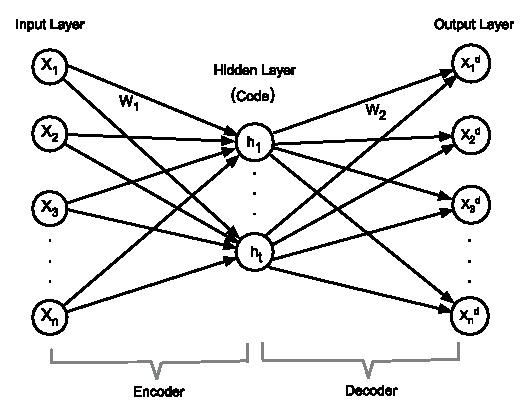
\includegraphics[width=.75\textwidth]{chapters/utility/img/ae_schema.eps}
\caption{Classical structure of an autoencoder. $X$ is the input data of the input layer, $h$ is the hidden layer's data, and $X^d$ is the reconstructed output data in the output layer.}
\label{fig:vae:ae_schema}
\end{figure}

\begin{lvae}

Recalling \autoref{ch:vae}, the essence of a variational autoencoder is that we take a variational distribution $q_\phi$ and choose the parameters $\phi$ to fit best the proposed distribution $p(\bZ)$. We also fit the data likelihood to best reconstruct the input from the proposed latent space distribution. The loss is the variational lower bound, given by
\begin{equation}
\Ls(\theta,\phi;\bX,\bA)=-D_{KL}(q_\phi(\bZ|\bX,\bA), p_\theta(\bZ))+\mathbb{E}_{q_\phi}\left[\log p_\theta(\bA|\bZ)\right]
\end{equation}

\end{lvae}

\chapter{Conclusion}
\label{ch:conclusion}

Lorem ipsum dolor sit amet, consectetur adipiscing elit. Fusce vulputate efficitur tellus ut consectetur. Aliquam erat volutpat. Morbi nulla nibh, bibendum cursus sem id, congue tempor quam. Aenean pulvinar lacus eget venenatis vestibulum. Sed in felis ac nulla ornare rutrum. Nunc placerat lobortis ultricies. Curabitur tortor felis, malesuada at ullamcorper sit amet, interdum sed erat. Duis ut pellentesque ante, quis tincidunt sapien. Nulla eu lectus nec enim rutrum egestas. In vulputate augue vitae enim tempus, a molestie elit mattis. Fusce porttitor, sem vel convallis sollicitudin, est nisi luctus mi, non suscipit lacus lorem quis libero. Sed leo mi, vehicula in ligula in, scelerisque laoreet justo. Sed tincidunt metus enim, non consectetur mi finibus ut. Nam at quam risus. Donec pharetra ante id leo faucibus blandit.

Lorem ipsum dolor sit amet, consectetur adipiscing elit. Nullam commodo rutrum tortor sit amet congue. Phasellus dolor ante, egestas id nibh luctus, lacinia aliquet nibh. Donec non arcu lacus. Donec nunc ligula, venenatis ut congue ullamcorper, pellentesque sed lorem. Nunc ornare hendrerit ipsum nec ultricies. Aenean posuere vel ex quis bibendum. Vestibulum malesuada diam mauris, tincidunt scelerisque velit feugiat quis.

Suspendisse dictum a neque nec vestibulum. Praesent faucibus tristique erat, eu finibus enim pharetra eu. Etiam id odio ut turpis accumsan accumsan et ut lectus. Pellentesque malesuada risus eget faucibus cursus. In hac habitasse platea dictumst. Pellentesque habitant morbi tristique senectus et netus et malesuada fames ac turpis egestas. Maecenas eget eleifend urna.

Donec vehicula metus non nisi tempus ornare. Pellentesque tristique dolor metus, malesuada imperdiet nibh cursus ut. Vivamus tellus neque, facilisis quis magna nec, dapibus mattis velit. Cras et odio ac odio egestas sagittis non vel tortor. Donec consectetur fringilla nisl, vitae tristique ligula consectetur id. Nunc quis lacinia arcu. Sed neque dolor, vehicula at tempus ut, placerat at turpis. Maecenas eget tempus odio. Etiam nunc nisi, convallis posuere nibh id, mattis faucibus libero. Proin porttitor, massa ut rhoncus sagittis, magna mi vehicula est, ac sodales arcu lacus vel mauris. Maecenas consectetur lectus commodo purus dictum malesuada.

Maecenas finibus mi at lacus molestie, at finibus arcu sagittis. Maecenas magna enim, aliquet vitae ante et, tristique efficitur odio. Vestibulum ante ipsum primis in faucibus orci luctus et ultrices posuere cubilia curae; Etiam in egestas leo. Nullam dapibus sodales eros, id varius sem varius in. Fusce interdum semper tempor. Duis imperdiet euismod risus, pretium malesuada est ornare at. Proin euismod est sit amet elementum viverra. Donec tincidunt eu purus non ultricies.



% 
%==============================================================

\backmatter

\bibliography{Thermo_paper_bib}
\bibliographystyle{acm}


\end{document}
